%%%%%%%%%%%%%%%%%%%%%%%%%%%%%%%%%%%%%%%%%
% Beamer Presentation
% LaTeX Template
% Version 1.0 (10/11/12)
%
% This template has been downloaded from:
% http://www.LaTeXTemplates.com
%
% License:
% CC BY-NC-SA 3.0 (http://creativecommons.org/licenses/by-nc-sa/3.0/)
%
%%%%%%%%%%%%%%%%%%%%%%%%%%%%%%%%%%%%%%%%%

%----------------------------------------------------------------------------------------
%	PACKAGES AND THEMES
%----------------------------------------------------------------------------------------

\documentclass[handout]{beamer}

\mode<presentation> {

% The Beamer class comes with a number of default slide themes
% which change the colors and layouts of slides. Below this is a list
% of all the themes, uncomment each in turn to see what they look like.

%\usetheme{default}
%\usetheme{AnnArbor}
%\usetheme{Antibes}
%\usetheme{Bergen}
%\usetheme{Berkeley}
%\usetheme{Berlin}
%\usetheme{Boadilla}
%\usetheme{CambridgeUS}
%\usetheme{Copenhagen}
%\usetheme{Darmstadt}
%\usetheme{Dresden}
%\usetheme{Frankfurt}
%\usetheme{Goettingen}
%\usetheme{Hannover}
%\usetheme{Ilmenau}
%\usetheme{JuanLesPins}
%\usetheme{Luebeck}
\usetheme{Madrid}
%\usetheme{Malmoe}
%\usetheme{Marburg}
%\usetheme{Montpellier}
%\usetheme{PaloAlto}
%\usetheme{Pittsburgh}
%\usetheme{Rochester}
%\usetheme{Singapore}
%\usetheme{Szeged}
%\usetheme{Warsaw}

% As well as themes, the Beamer class has a number of color themes
% for any slide theme. Uncomment each of these in turn to see how it
% changes the colors of your current slide theme.

%\usecolortheme{albatross}
%\usecolortheme{beaver}
%\usecolortheme{beetle}
%\usecolortheme{crane}
%\usecolortheme{dolphin}
%\usecolortheme{dove}
%\usecolortheme{fly}
%\usecolortheme{lily}
%\usecolortheme{orchid}
%\usecolortheme{rose}
%\usecolortheme{seagull}
%\usecolortheme{seahorse}
%\usecolortheme{whale}
%\usecolortheme{wolverine}

%\setbeamertemplate{footline} % To remove the footer line in all slides uncomment this line
%\setbeamertemplate{footline}[page number] % To replace the footer line in all slides with a simple slide count uncomment this line

%\setbeamertemplate{navigation symbols}{} % To remove the navigation symbols from the bottom of all slides uncomment this line
}

\usepackage{graphicx} % Allows including images
\usepackage{booktabs} % Allows the use of \toprule, \midrule and \bottomrule in tables
\usepackage{cool}
\usepackage{tikz}
\usepackage{amsmath}
\usepackage{xcolor}
\usepackage{hyperref}
\usepackage{bm}

\DeclareMathOperator*{\argmax}{argmax}
\DeclareMathOperator*{\argmin}{argmin}
\usetikzlibrary{positioning}

%----------------------------------------------------------------------------------------
%	TITLE PAGE
%----------------------------------------------------------------------------------------

\title[AI for Digital Retail]{AI for Digital Retail} % The short title appears at the bottom of every slide, the full title is only on the title page

\author{Ashwin Rao} % Your name
\institute[Stanford] % Your institution as it will appear on the bottom of every slide, may be shorthand to save space
{Stanford University
 % Your institution for the title page
}

\date{} % Date, can be changed to a custom date

\begin{document}
\begin{frame}
\titlepage % Print the title page as the first slide
\end{frame}

% \begin{frame}
% \frametitle{Overview} % Table of contents slide, comment this block out to remove it
% \tableofcontents % Throughout your presentation, if you choose to use \section{} and \subsection{} commands, these will automatically be printed on this slide as an overview of your presentation
% \end{frame}


\begin{frame}
\frametitle{A bit about me}
\pause
\begin{itemize}[<+->]
\item Co-Founder of CX Score: AI to enhance Digital Customer Experience
\item Adjunct Professor, \href{https://icme.stanford.edu/}{\underline{\textcolor{blue}{Applied Mathematics (ICME)}}}, Stanford University
\item Past: VP of AI at Target Corporation (ML for Operations and Digital)
\item Past: MD at Morgan Stanley, Trading Strategist at Goldman Sachs
\item I direct Stanford's \href{https://mcf.stanford.edu/}{\underline{\textcolor{blue}{Mathematical \& Computational Finance program}}}
\item Research \& Teaching in: {\em RL and it's applications in Finance \& Retail}
\item Book:  \href{https://www.amazon.com/Foundations-Reinforcement-Learning-Applications-Finance/dp/1032124121}{\underline{\textcolor{blue}{Foundations of RL with Applications in Finance}}}
\item CX Score: AI enabling retailers to deliver great Customer Experience
\end{itemize}
\end{frame}


\begin{frame}
\frametitle{Machine Learning Branches}
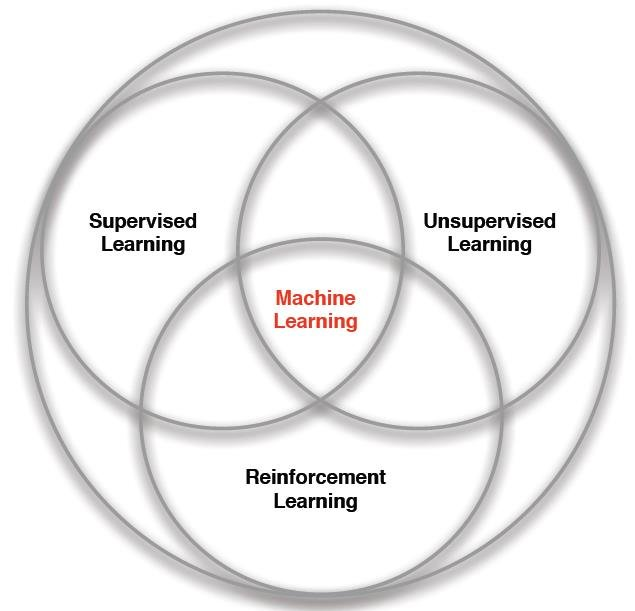
\includegraphics[width=9cm, height=8cm]{../finance/cme241/MLBranches.PNG}
\end{frame}

\begin{frame}
\frametitle{Machine Learning Overview}
\pause
\begin{itemize}[<+->]
\item ML is roughly classified into Supervised, Unsupervised and RL
\item Supervised: Predicts by learning relationships between variables
\item Unsupervised: Unearths patterns \& structures within data
\item RL: Optimal Sequential Decisioning under Uncertainty
\item ML has been a breakthrough for images, text, games
\item Largely due to the past decade of success of Deep Neural Networks
\item We are now adapting Deep Learning techniques to other domains
\item Works well when we have plenty of data and plenty of compute
\item ML practice tends to be quite laborious on Big Data Engineering
\item I've seen promising results in Finance and Retail applications
\end{itemize}
\end{frame}


\begin{frame}
\frametitle{AI for Digital Customer Engagement \& Profitability}
\pause
\begin{itemize}[<+->]
\item AI has been used extensively in Digital Retail
\item Primarily for Search, Recommendations, Marketing/Ads
\begin{itemize}
\item Search Relevance - Language Models, Product  {\em Embeddings}
\item Personalized Recommendations/Ads - Customer  {\em Embeddings}
\item Tactical Promotion of Products (eg: Profitability, Inventory, Clearance)
\end{itemize}
\item Moving on to personalizing/optimizing entire page content/structure
\item Natural progression to personalizing/optimizing web/mobile {\em journeys}
\item Balancing multiple objectives of customer engagement \& profitability
\item Techniques: {\em Multi-Armed Bandits} and {\em Reinforcement Learning}
\end{itemize}
\end{frame}


\begin{frame}
\frametitle{Similar/Substitutable Products identified with {\em Embeddings}}
\pause
\begin{itemize}[<+->]
\item {\em Embeddings} automate identification of similarity/substitutability
\item Similarity by Visuals or by Descriptions or by Customer Interest
\item Throw this heterogeneous data into deep neural network learning
\item Deep inside the neural network, we find encodings of these products
\item Similar/Substitutable products have similar encodings
\item The technical term for these encodings is \href{https://developers.google.com/machine-learning/crash-course/embeddings/video-lecture}{\underline{\textcolor{blue}{Embeddings}}}
\item Embeddings are low-dimensional numerical representations ({\em Vectors})
\item Capturing the most important features of products
\item Captures various relationships between products, eg: complementarity
\item Based on product images, descriptions, customer interest
\item Embeddings can be used as ML features for transfer learning
\item Embedding vectors have powerful algebraic/geometric properties
\end{itemize}
\end{frame}

\begin{frame}
\frametitle{Book Embeddings flattened to 2-D Vectors}
\includegraphics[width=12cm, height=8cm]{../supply_chain/BookEmbeddings.png}
\end{frame}




\begin{frame}
\frametitle{RL for Optimized Web/Mobile Journeys}
\pause
\begin{itemize}[<+->]
\item Today almost all retail companies use ML for Personalization
\item Product Recommendations/Marketing based on customer interest
\item So product displays are customized to generate clicks/engagement
\item Uses Customer Embeddings and Contextual Bandits techniques
\item Now this is being extended to personalizing the entire page
\item The natural progression is to personalize web/mobile journeys
\item Objective is to blend customer engagement \& profitability
\item Core Problem: Optimal Sequential Decisioning under Uncertainty
\item This problem cries out for Reinforcement Learning (RL)
\item RL based on the powerful framework of Markov Decision Processes
\end{itemize}
\end{frame}

\begin{frame}
\frametitle{The \href{https://en.wikipedia.org/wiki/Markov_decision_process}{\underline{\textcolor{yellow}{Markov Decision Process}}} Framework}
\includegraphics[width=12cm, height=7cm]{../finance/cme241/MDP.png}
\end{frame}


\begin{frame}
\frametitle{Components of the MDP Framework}
\pause
\begin{itemize}[<+->]
\item The {\em Agent} and the {\em Environment} interact in a time-sequenced loop
\item {\em Agent} responds to [{\em State}, {\em Reward}] by taking an {\em Action}
\item {\em Environment} responds by producing next step's (random) {\em State}
\item {\em Environment} also produces a (random) number we call {\em Reward}
\item Goal of {\em Agent} is to maximize {\em Expected Sum} of all future {\em Reward}s
\item By controlling the ({\em Policy} : {\em State} $\rightarrow$ {\em Action}) function
\item This is a dynamic (time-sequenced control) system under uncertainty
\item MDP framework enables modeling problem of optimized app journeys
\end{itemize}
\end{frame}

\begin{frame}
\frametitle{How a baby learns to walk}
\includegraphics[width=13cm, height=8cm]{../finance/cme241/BabyMDP.jpg}
\end{frame}

\begin{frame}
\frametitle{Many real-world problems fit this MDP framework}
\pause
\begin{itemize}[<+->]
\item Self-driving vehicle (speed/steering to optimize safety/time)
\item Game of Chess (Boolean {\em Reward} at end of game)
\item Inventory Replenishment to ensure high availability at low cost
\item Make a humanoid robot walk/run on difficult terrains
\item Manage an investment portfolio (covered in depth in my book)
\item Control a power station
\item Hyper-Personalized Apps for optimizing user engagement
\item Optimal decisions during a football game
\item Strategy to win an election (high-complexity MDP)
\end{itemize}
\end{frame}

\begin{frame}
\frametitle{Self-Driving Vehicle}
\includegraphics[width=13cm, height=8cm]{../finance/cme241/CarMDP.jpg}
\end{frame}

\begin{frame}
\frametitle{Web/Mobile Journey Optimization as an MDP}
\pause
\begin{itemize}[<+->]
\item MDP {\em State} is past and current data from the customer
\item {\em State} also includes location, trends, pricing, inventory etc.
\item {\em Action} is the content and structure of next page to display
\item {\em Reward} function blends customer engagement and profitability
\item State transitions governed by uncertainty in customer "clicks"
\item Solve: \href{https://en.wikipedia.org/wiki/Dynamic_programming}{\underline{\textcolor{blue}{Dynamic Programming}}} or
 \href{https://en.wikipedia.org/wiki/Reinforcement_learning}{\underline{\textcolor{blue}{Reinforcement Learning}}}
\item Curse of Dimensionality and Curse of Modeling $\Rightarrow$ RL
\end{itemize}
\end{frame}


\begin{frame}
\frametitle{How RL Works: Learning from Samples of Data}
\pause
\begin{itemize}[<+->]
\item RL incrementally learns from state/reward transitions data
\item Typically served by a simulator acting as a {\em Simulated Environment}
\item RL is a ``trial-and-error'' approach linking {\em Actions} to {\em Rewards}
\item Try different actions \& learn what works, what doesn't
\item Deep Neural Networks are typically used for function approximation
\item Big Picture: Sampling and Function Approximation come together
\item RL algorithms are clever about balancing  ``explore'' versus ``exploit''
\item Promise of modern A.I. is based on success of RL algorithms
\item Potential for automated decision-making in many industries
\item In 10-20 years: Bots that act or behave more optimal than humans
\item RL already solves various low-complexity real-world problems
\item RL has many applications in Retail, in Operations and Digital
\item RL covered in detail in my book, with applications in Finance/Retail
\end{itemize}
\end{frame}

\end{document}